\RequirePackage[2020-02-02]{latexrelease}
\documentclass[letter,scriptaddress,twocolumn, prl]{revtex4}

\usepackage{amsmath}%,amssymb} 
\usepackage{makeidx}
\usepackage{amsfonts}
\usepackage[ansinew]{inputenc}
%\usepackage[usenames,dvipsnames]{pstricks}
%\usepackage{subfigure}
\usepackage{epsfig}
\usepackage{float}
%\usepackage{pst-grad} % For gradients
%\usepackage{pst-plot} % For axes
\usepackage[colorlinks,hyperindex]{hyperref}
\hypersetup
{
colorlinks,%
citecolor=black,%
linkcolor=black,%
urlcolor=black,%
}

\setlength\textheight{24.5cm}

% --- Comandos novos ---
\newcommand{\dket}[1]{\left| #1 \right)}
\newcommand{\E}[1]{\frac{\hbar^2 #1 ^2}{2m_0}}
\newcommand{\dbra}[1]{\left( #1 \right|}
\newcommand{\dsubmin}[1]{\left( #1 \right)}
\newcommand{\dbraket}[2]{\left( #1 | #2 \right)}
\newcommand{\dbraketm}[3]{\left( #1 \left| #2 \right| #3 \right)}
\newcommand{\ket}[1]{\left| #1 \right\rangle}
\newcommand{\bra}[1]{\left\langle #1 \right|}
\newcommand{\submin}[1]{\left\langle #1 \right\rangle}
\newcommand{\braket}[2]{\left\langle #1 \right. \left| #2 \right\rangle}
\newcommand{\braketm}[3]{\langle #1 \mid #2 \mid #3 \rangle}
\newcommand{\pinterno}[2]{\left( #1 , #2 \right)}
\newcommand{\comut}[2]{\left[ #1 , #2 \right]} % THE COMUTATOR
\newcommand{\seitz}[2]{\left\{ \, #1 \mid  #2 \, \right\}}
\newcommand{\rep}{\emph{rep} }
\newcommand{\irep}{\emph{irrep} }
\newcommand{\ordem}[1]{\mid #1 \mid}
\newcommand{\op}[1]{\mathbb #1 }
\newcommand{\group}[1]{\mathcal #1 }
\newcommand{\vet}[1]{\mathbf #1 }
\newcommand{\argu}[1]{\left( #1 \right)}
\newcommand{\kp}{\vet{k}\cdot\vet{p}}

\makeindex

%--------------------------------------------------------
\begin{document}

\title{Computational Simulation of the 2d Ising Model}

\author{Alex Roseman}
\author{Adrian Hall}
\date{\today}

\begin{abstract}
Dear all: apologies for this mess of a first draft. We ran into some conceptual problems late today (autocorrelation asymptotically approaches negative values even after B annealing/lattice snapshot sanity checks). In general, our calculated values for Tc and the critical exponents are often several sigma away from analytic values. We don't think the issue is error analysis: our uncertainties seem to reflect the variation in the data, and so we think there is some more fundamental issue with the underlying data. As far as we can tell, this issue is NOT the number of steps, the lattice size, macroscopic domains at low temperatures, or the number of independent simulations.
\end{abstract}

\maketitle

\begin{figure*}[t]
	\begin{center}
		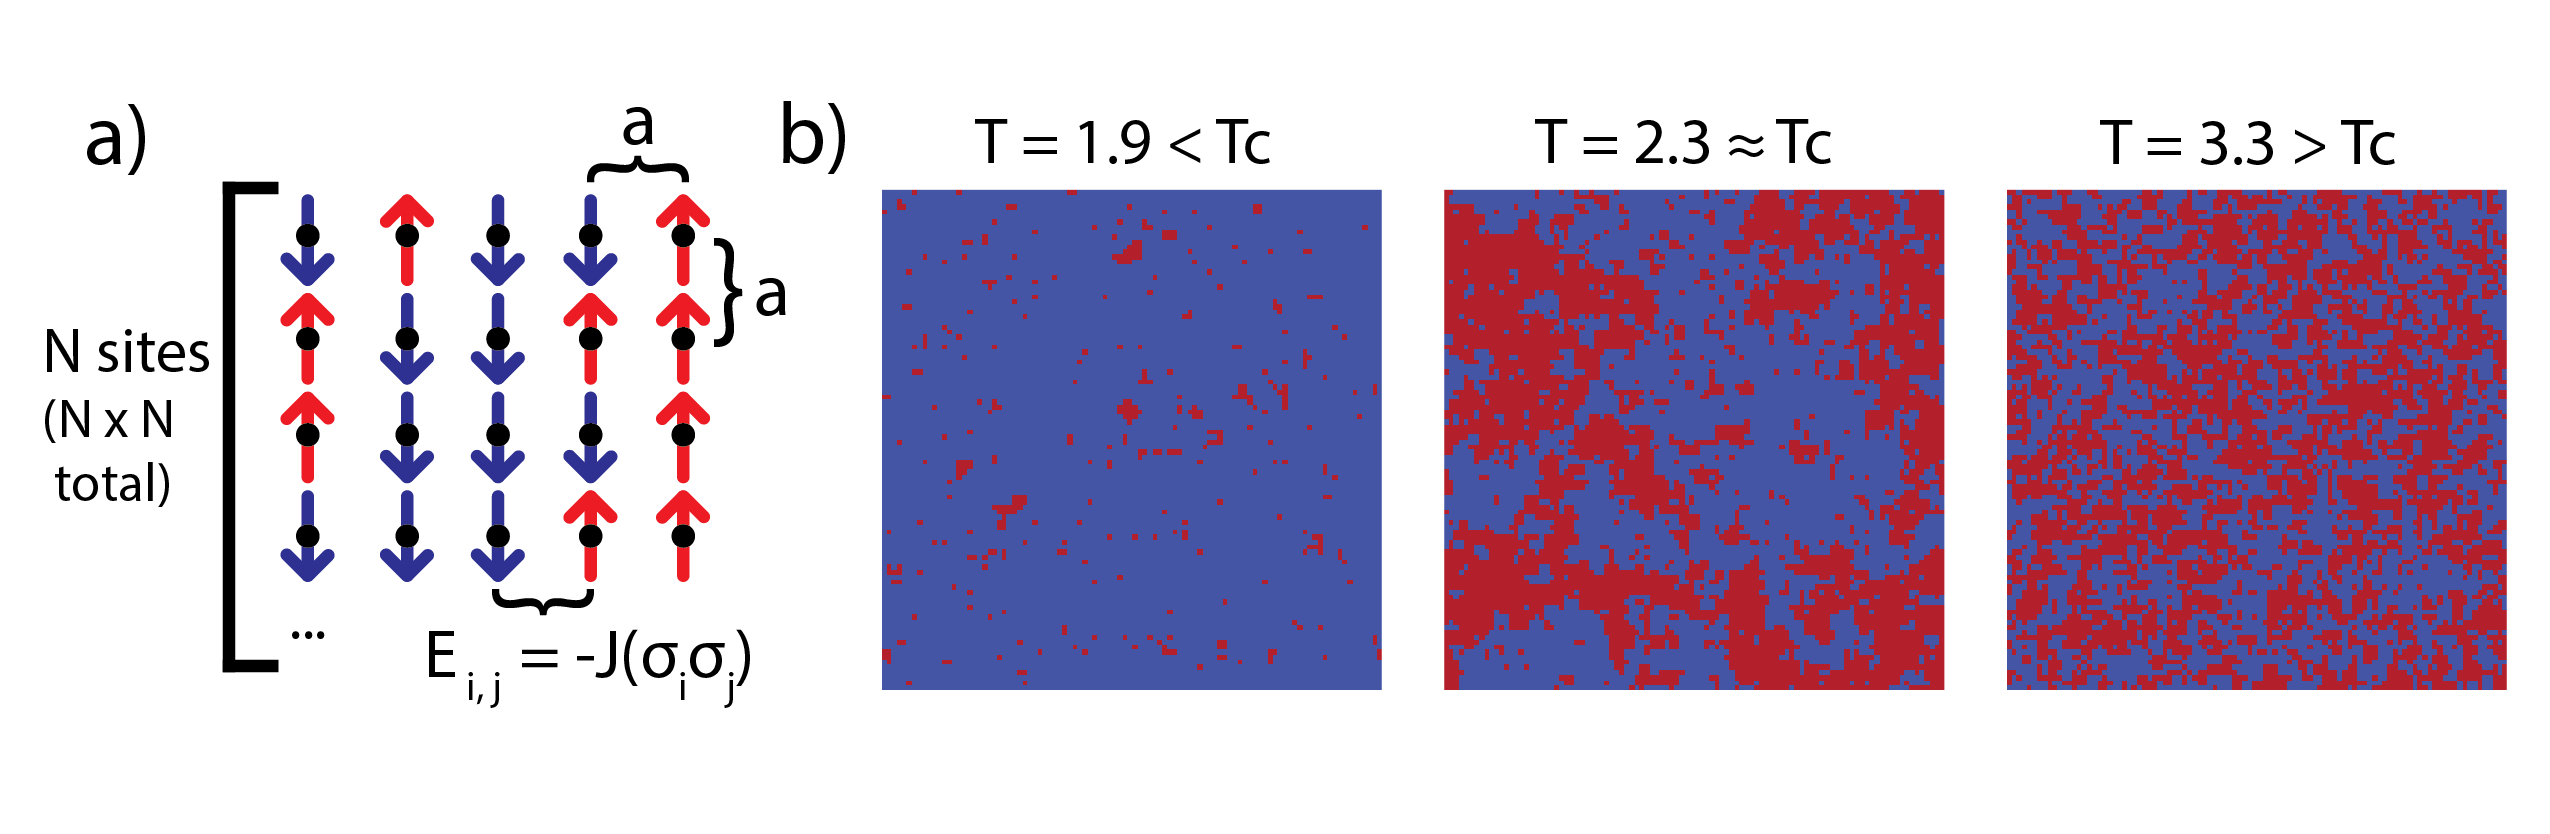
\includegraphics[width=1\textwidth]{figs/fig1.png}
		\caption{a. diagram of the lattice. We use N=100 throughout. $E_{i, j}$ is neighbor spin interaction - adjacents only, wraps (each site has 4 neighbors). "a" is lattice distance (1), J = 1, spin = $\pm 1$. b. Snapshots after ~10 million simulation steps at the given temperature, showing typical states below, near, and above Tc. Red is spin up, blue spin down.}
		\label{fig:fig1}
	\end{center}
\end{figure*}

\section{Introduction}

The 2d Ising Model consists of a two-dimensional square lattice of $N^2$ particles, each with spin $\sigma_i = \pm1$. The particles interact with one another through nearest-neighbor interactions of strength J, and with an external magnetic field of strength B, and the whole system has Hamiltonian:

\begin{equation}
	\label{eq:hamiltonian}
	H = -J \sum_{\left\langle i, j \right\rangle}\sigma_i\sigma_j - B \sum_i\sigma_i
\end{equation}

where $\sigma_i$ is the spin state of the $i$-th particle, and the interaction energy is a sum over nearest neighbors. Each particle has four nearest neighbors, and the lattice wraps around, so that the first particle in a given row is neighbors with the second and the $N$-th. The lattice is depicted in \autoref{fig:fig1}, a.

The Ising Model is notable in that it has an analytic solution, first found by [[Onsager in...]] in the limit $N\rightarrow\infty$. The 2d Ising Model also has a phase transition, which for $B = 0$ and $N\rightarrow\infty$ occurs at critical temperature:

\begin{equation}
	\label{eq:Tc}
	T_c = \frac{2}{\ln{(1+\sqrt{2})}} \approx 2.269 (J/k_B)
\end{equation}

where J is the nearest-neighbor interaction energy as in Equation 1, and $k_B$ is the Boltzmann constant, so that $T_c$ is dimensionless overall. \autoref{fig:fig1}, b shows typical lattice states below, near, and above $T_c$.

These states were generated using a Markov-Chain Monte-Carlo (MCMC) simulation of the Ising Model. The physical probability of any overall lattice state is given by the Gibbs distribution, which states that the probability of finding a macroscopic system in a microscopic state of energy E is proportional to $e^{-\frac{E}{k_BT}}$. In this experiment, we reproduce this probabilities using Metropolis sampling. The lattice is initialized to a random state, with each $\sigma_i$ initialized to $1$ or $-1$. The lattice is then evolved for a number of steps, with each step as follows:
\begin{enumerate}
	\item Some number of lattice sites (i.e. particles) are selected randomly (in our simulation, this number was ten percent of the total lattice).
	\item We calculate the overall change in energy from flipping the spin of each selected particle, $\Delta E_i = 2(J\sigma_i(\sum_j\sigma_j) + B\sigma_i)$, where $\sigma_i$ is the flipped spin of the particle, and $\sigma_j$ are the spins of the particle's four neighbors.
	\item The spin at each selected lattice site is or is not flipped depending on $\Delta E_i$ (the calculation is independent for each site).
	\begin{enumerate}
		\item if $\Delta E < 0$, the spin is flipped.
		\item if $\Delta E > 0$, the spin is flipped with probability $e^{-\Delta E_i/(k_BT)}$
	\end{enumerate}
\end{enumerate}

This approximately reproduces the Gibbs distribution, approaching the distribution exactly as the numbers of steps approaches infinity.

[[Could discuss flip percentage here. also convergence (point to appendix)]]

[[Next and last: quantities and units. Plan: quantities, then units (and dimensionless quantities), then explanation of the functions we fit to]]

\begin{itemize}
	\item Ising Model: Electrons have spin, interact w. overall field and nearest neighbors (adjacent) $H = -J \Sigma \sigma_i \sigma_j - B\Sigma \sigma_i$. See Fig. 1
	\item 2d lattice is rare model with both phase transition and an analytic solution (cite Onsager paper), in the limit N$\rightarrow\infty$. 
	\item Can simulate with MCMC metropolis sampling. Probability of any given state from Gibbs dist: $P \sim e^{-\frac{E}{k_BT}}$, Metropolis proxies this by spending time in each state proportional to its probability. 
	\subitem [Give algorithm for $P_{flip}$ here, and explain Goldilocks zone of flipping just the right number of sites: too many and you lose some effect of neighbor spin interactions. Too few and you never get anywhere]. 
	\subitem Needs time to find the typical set, which you can accelerate with annealing. Needs enough time \textit{in} the typical set to get a representative sample (see appendix on convergence).
	\item introduce quantities: $<M>$ and $<E>$ (see fig: 2), $\chi$ and $c_V$ (fig 3), auto-correlation and $\xi$ (fig 4). Explain auto-correlation subtracting mean spin in each row/column (think about example case of ~all spin up with a tiny pocket of spin down - that pocket is way more important than all the perfect spin up correlations).
	\subitem Can find specific heat and susceptibility through the variance in E and M (show partition function math? Or just cite it as well-known)
	\subitem $\xi$ indicates that N=100 lattice is reasonable approximation for infinite lattice
	\item \textbf{Units:} Explain "unitless" units. Ours have tildes
	\subitem "$J = 1$", unitless spin and thus magentization
	\subitem $\tilde{E} = E/J$, $\tilde{T} = k_BT/J$, $\tilde{M} = M $
	\subitem $\beta = \frac{1}{k_BT} = \frac{1}{J\tilde{T}}$
	\subitem $P \sim e^{-\frac{E}{k_BT}} = e^{-\frac{\tilde{E}}{\tilde{T}}}$
	\subitem $c_V = \frac{\beta}{T}(\left\langle E^2 \right\rangle - \left\langle E \right\rangle ^2)$. $\tilde{c}_V = c_V / k_B = \frac{1}{\tilde{T}^2}(\left\langle \tilde{E}^2 \right\rangle - \left\langle \tilde{E} \right\rangle ^2)$
	\subitem $\chi = \beta(\left\langle M^2 \right\rangle - \left\langle M \right\rangle ^2)$. $\tilde{\chi} = J\chi = \frac{1}{\tilde{T}}(\left\langle \tilde{M}^2 \right\rangle - \left\langle \tilde{M} \right\rangle ^2)$
	\item Explain critical exponents. List analytic values and identities.
	\item Subtle points (to remember to include): 
	\subitem the lattice wraps around. 
	\subitem The simulation outputs E as energy per lattice site, and M as magnetization per site. In variance, this ends up squared, so you need an additional factor of $N^2$ to get the units right for $\chi$ and $c_V$, which should have factors of $N^{-2}$, not $N^{-4}$, and should not depend on lattice size)
\end{itemize}

\section{Data and Analysis}
\begin{itemize}
	\item Simulation parameters: N = 100, 3000 steps sloping down linearly from T = 4.0, B = 0.5 to T = final temp (x axis in graphs), B=0. Then 5000 steps of burn-in and 100,000 steps of taking data (see convergence appendix for why these numbers). Flip percentage: 10\% (a default value which we didn't have time to examine).
	\item The critical exponent power laws are valid "near the critical temperature". We have a well-reasoned inner bound, based on convergence being harder to achieve closer to Tc, but we don't have solid logic for the outer bound being where it is. Too close to Tc and there's not enough data. Too far and the tail end of the fit gets way too much weight.
	\item We calculate Tc and critical exponents using Scipy's curve fit function, which generates parameters (using the Levenberg-Marquardt algorithm) to minimize least squares error (i.e. minimize $\chi^2$). Uncertainty in these parameters is calculated using Scipy's covariance matrix. We intend to write a more complete explanation of the precise origin of these error estimates. We will also do a standard $\chi^2$ test on all fits, to get a sense of how accurate they are.
\end{itemize}

\begin{figure}[h]
	\begin{center}
		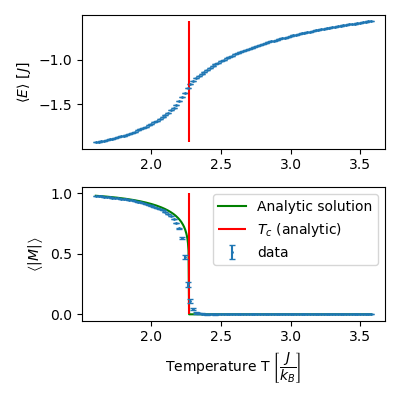
\includegraphics[width=.5\textwidth]{figs/fig2_EMplots.png}
		\caption{Mean energy (top) and absolute magnetization (bottom) per lattice site as computed by MCMC simulation at a range of temperatures. Data is drawn from 97 independent simulations: each data point is the average value of $\left\langle M \right\rangle$ over all simulations; each standard error is the standard error of the mean of $\left\langle M \right\rangle$ over all simulations, treating each $\left\langle M \right\rangle$ as an independent measurement. Analytic Tc (red) and analytic curves (green) plotted for comparison. At first glance, our system appears to reach phase transition at lower temperature than the analytic $T_c$.}
		\label{fig:fig2}
	\end{center}
\end{figure}



\begin{figure}[h]
	\begin{center}
		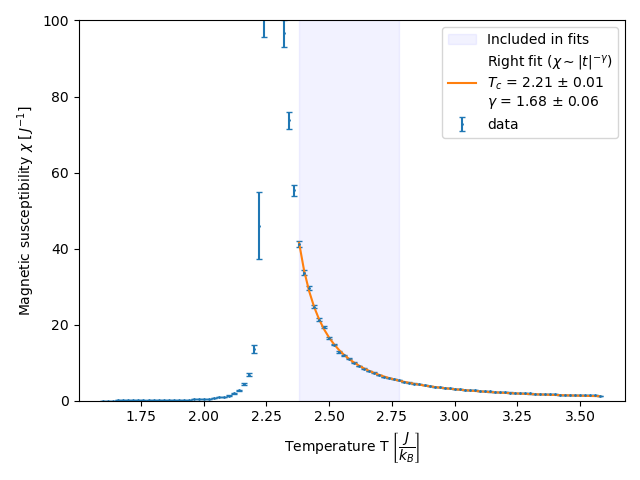
\includegraphics[width=.4\textwidth]{figs/fig3_chi.png}
		\caption{Magnetic susceptibility at a range of temperatures. Susceptibility is calculated from variance in M over each simulation, which is taken as a single measurement. Data points on this graph are the mean of variance(M) over all 97 simulations at a given temperature, and error bars on this graph are the standard error of this mean. Shown in orange is a power law fit with $T_c$ and $\gamma$ considered as free variables, using only the data in the shaded column. NOTE: we intend to merge figures 3 and 4 into a single figure with 2 graphs.}
		\label{fig:fig3a}
	\end{center}
\end{figure}
\begin{figure}[h]
	\begin{center}
		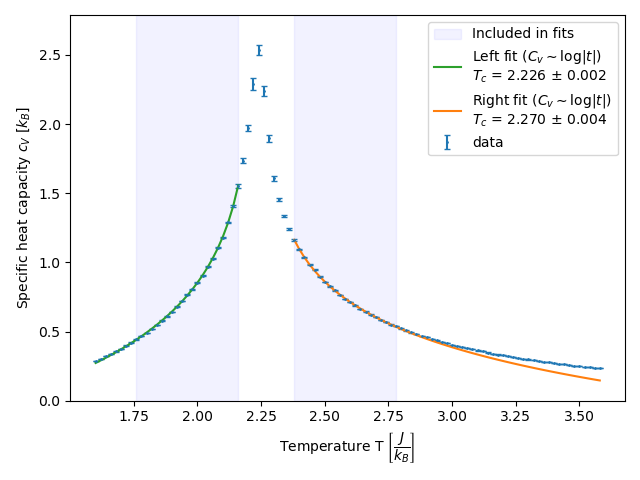
\includegraphics[width=.4\textwidth]{figs/fig3_cv.png}
		\caption{Specific heat at a range of temperatures. Like susceptibility, specific heat is calculated from variance in E across MCMC steps. Data points on this graph are the mean of variance(E) over all 97 independent simulations at a given temperature, and error bars on this graph are the standard error of this mean. Shown in orange and green are logarithmic fits in which $T_c$ was considered a free variable, using only the data in the shaded columns. We generated separate fits on the left and right of Tc. Although the power law should be symmetric, we find significantly different results for Tc. NOTE: we intend to merge figures 3 and 4 into a single figure with 2 graphs.}
		\label{fig:fig3b}
	\end{center}
\end{figure}
\begin{figure}[h]
	\begin{center}
		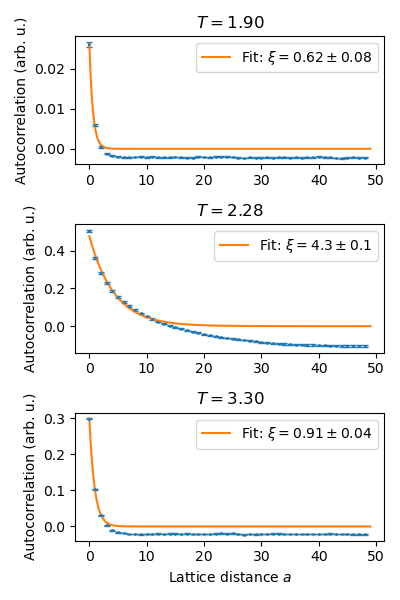
\includegraphics[width=.4\textwidth]{figs/fig4_autocors.png}
		\caption{Autocorrelation functions at representative temperatures: below, near, and above $T_c$. Shown in orange are exponential decay functions fit by least-squares regression to the positive portion of the autocorrelation data, with length scale parameter $\xi$. Autocorrelation seems to become negative (i.e. anticorrelated) after sufficient lattice distance, leading the exponential fit to deviate significantly from the data. This likely plays a role in our terrible estimate for $\nu$. Note: we intend to merge Figs. 5 and 6.}
		\label{fig:fig4a}
	\end{center}
\end{figure}
\begin{figure}[h]
	\begin{center}
		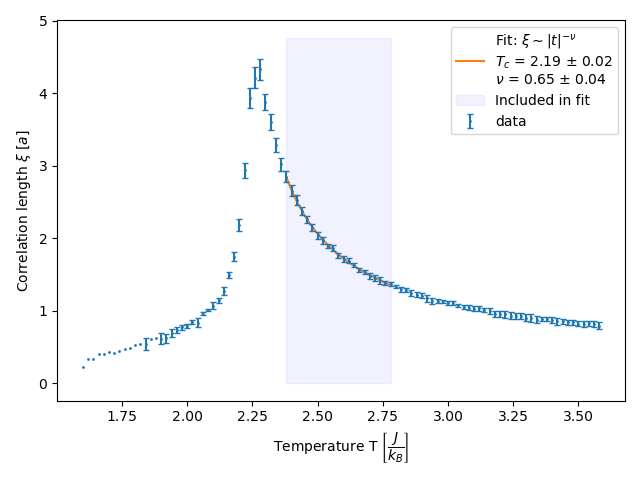
\includegraphics[width=.4\textwidth]{figs/fig4_xi.png}
		\caption{Correlation length $\xi$ at a range of temperatures. These data points are drawn from the fits depicted in Fig. 5, with all the inaccuracy that entails. Uncertainties are drawn from Scipy's curve fit covariance matrix. We intend to include a complete description of the nature of these uncertainties in the body of our report. As with $\chi$ and $c_v$, we fit a power law function (orange) to the data in the shaded region, with $T_c$ and $\nu$ as free parameters. Note: we intend to merge Figs. 5 and 6.}
		\label{fig:fig4b}
	\end{center}
\end{figure}
\begin{figure*}[h]
	\begin{center}
		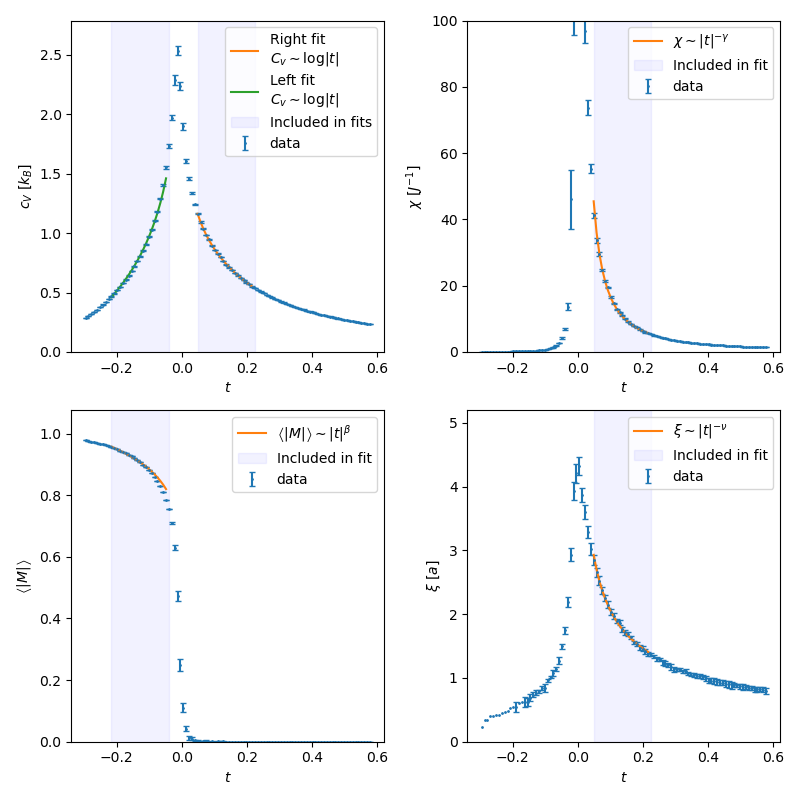
\includegraphics[width=1\textwidth]{figs/fig5_crit_exponents.png}
		\caption{Power law fits for the critical exponents for $c_V$ ($\alpha$) (upper left), $\chi$ ($\gamma$) (upper right), $|M|$ ($\beta$) (lower left), and $\xi$ ($\nu$) (lower right). We attempt to show $\alpha = 0$ by successfully fitting a logarithmic function to $c_V$. In each graph, the x-axis is the normalized temperature $t = \frac{T - T_c}{T_c}$, where $T_c$ is the analytic value of $T_c$. As before, only data from the shaded regions was used for fits. We find the following values: $\gamma = 1.40 \pm .01$, $\beta = 0.103 \pm .002$, $\nu = 0.49 \pm .01$. All critical exponents are, of course, unitless. We have not checked identities because these values are clearly broken, $\nu$ especially (see abstract for details).}
		\label{fig:fig5}
	\end{center}
\end{figure*}

%\begin{equation}
%	\label{eq:test}
%	\vec{f} = m \vec{a} .
%\end{equation}
%So, equation \eqref{eq:test} or \ref{eq:test} must be solved for position function so one can know everything about the system. But how to solve this. Here, $\vec{f}$ is a sum over all the forces acting on this particle, $\sum\limits_{\forall i} f_i$.
%In my books.bib, I have an entry named goldstein80 wich refers to Classical Mechanics by Goldstein. The same for greene1995.

% Fig.\,\ref{fig:example}.

%\begin{figure}[htbp]
%	\begin{center}
%		\includegraphics[width=0.3\textwidth]{exampleFig} %depending on the latex compiler, you can omit the file extension
%		\caption{Include your caption here.}
%		\label{fig:example}
%	\end{center}
%\end{figure}

\section{Acknowledgements}
	Prof. Navon, Prof. Newburgh, HongJoon

\bibliographystyle{unsrt} 
%\bibliography{/home/thiago/bibtex/articles,/home/thiago/bibtex/books}

\begin{thebibliography}{}
	
	\bibitem{Onsager}
	Lars Onsager,
	\textit{Crystal Statistics. I. A Two-Dimensional Model with an Order-Disorder Transition},
	Physical Review {\bf 65}, 117 (1944).
	
	
\end{thebibliography}

\appendix
\section{\\Appendix A: Convergence}
We intend to write an appendix concerning the aspects of convergence we have previously discussed with Prof. Newburgh and Prof. Navon: how many steps are required to get a representative slice of the typical set. Of the values we calculate, the most affected here are $\chi$ and $c_V$. While the simulation reaches the typical set fairly quickly, it takes quite a while (order $10^5$ steps) to reach values of $\left\langle M^2 \right\rangle - \left\langle M \right\rangle ^2$ and $\left\langle E^2 \right\rangle - \left\langle E \right\rangle ^2$ which no longer scale as more steps are added. We choose our number of steps parameter in the simulation to give converged values of variance outside of radius $r = .1$ from analytic $T_c$, then exclude data within this radius throughout our analysis. When we submit our final report, Fig. 8 will be cleaned up, and the analogous data for E will be plotted or explained, depending on whether the E data looks qualitatively different.

ABout fig 8: The data points graphed here take each group's variance as an individual measurement (as if we had run independent simulations of that many steps). For example, with $n_{steps} = 10,000$, the total million steps were split into 200 groups of 10,000 steps each. A variance was then calculated for each group. The data point at x = 10,000 is the average of these variances, and the error bar at x = 10,000 is the standard error of this mean. There is no error bar at x = 1,000,000 because the data was split into only a single group.

\begin{figure}[h]
	\begin{center}
		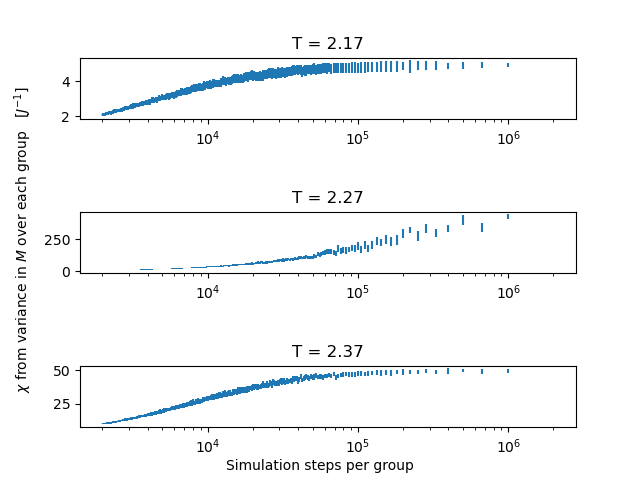
\includegraphics[width=.4\textwidth]{figs/figA1.png}
		\caption{$\chi$ values calculated with data from a simulation of 2,000,000 analyze steps. The total 2,000,000 steps were split as evenly as possible into groups of $n_{steps}$ (x axis), and variance in M was calculated across each group. Each data point is the average variance over all such groups.}
		\label{fig:figA1}
	\end{center}
\end{figure}

\end{document}
